\documentclass{article}
\usepackage{amsmath,amsthm,amssymb}
\usepackage{mathtools}
\usepackage{graphicx}
\usepackage[utf8]{inputenc}
\usepackage{enumitem}  
\usepackage{setspace}
\usepackage{ mathrsfs }
\usepackage{tikz}
\usepackage{array}
\usepackage{longtable}
\usetikzlibrary{arrows, shapes, backgrounds,fit}
\usepackage{tkz-graph}
\usepackage{color}
\usepackage{pgfplots}
\definecolor{deepblue}{rgb}{0,0,0.5}
\definecolor{purple}{rgb}{120,0,130}
\definecolor{deepgreen}{rgb}{0,0.5,0}
\onehalfspacing
\usepackage[a4paper,left=3cm,right=2cm,top=2.5cm,bottom=2.5cm]{geometry}
\begin{document}
\
\\
{\large $CSC336$}
\hfill{\large Rui Ji} \\
\null\hfill{\large $1000340918$}\\
\begin{center} 
\section*{\centering\textcolor{black} {Problem Set 1}}
\end{center}
\begin{enumerate}
\item 
	\begin{enumerate}
		\item In IEEE binary system, the single precision F (2, 24, L, U ) for a fixed exponent, since the first digit is always 1 then, there are $2^{23}$ different numbers. \\
			Similarly, in IEEE binary system, the double precision F (2, 53, L, U ) for a fixed exponent there are $2^{52}$ different numbers. \\
			Hence, there are $\frac{2^{52}}{2^{23}} - 1 = 2^{29} -1$ double precision numbers between any two adjacent nonzero single precision numbers
		\item In IEEE binary system, the double precision F (2, 53, L, U )  carries 53 bits;  hence, the largest $p$ for double is, $p =2^{53} -1$\\
			In IEEE binary system, the single precision F (2, 24, L, U )  carries 24 bits;  hence, the largest $p$ for single precision is, $p = 2^{24} -1$
	\end{enumerate}
\item 
	\begin{enumerate}
		\item The first loop prints 5 values of $a$, and the second loop prints 4 values of $b$.\\
			For the first loop we have:
			\begin{itemize} [label={}]
			 \item $0.1_2 =  0.0 \ \overline{0011}$; hence, in IEEE representation for double, 
			 \item $0.1 = 1.1 \ 0011...\ 0011 \ 01_{52} 0_{53} \times 2^{-4}$
			 \item $0.2 = (0.1+0.1)_2 = 1.10 \ 0110 \ 0110 ... \ 0110 \ 1_{52}0_{53} \times 2^{-3}$
			 \item $0.3 = (0.1+ 0.1+0.1)_2 = 1. 001 \ 1001 \ 1001 ... \ 1001 \ 1010_{52} \ 0_{53} \times 2^{-2}$
			 \item $0.4 = (0.1+0.1+0.1+0.1)_2 = 1.100 \ 1100 \ 1100 ... 1100\ 1101_{52} \ 0_{53} \times 2^{-2}$
			 \item $0.5 = (0.1+0.1+0.1+0.1+0.1)_2 = 1.0000 \ 0000 \ ...00_{52}0_{53} \times 2^{-1}$
			 \item Hence, the first loop print out 5 numbers. 	
			\end{itemize}
			For the second loop we have:
			\begin{itemize} [label={}]
			 \item $1.1_2 =  1.0 \ \overline{0011}$; hence, in IEEE representation for double,
			 \item $1.1 = 1.0 \ 0011...\ 0011 \ 01_{52} 0_{53} \times 2^{0}$
			 \item $1.2 = (1.1+0.1)= 1.0 \ 0110 \ 0110 ... \ 0110 \ 10_{52}0_{53} \times 2^{0}$
			 \item $1.3 = (1.1 + 0.1+0.1) = 1. 0 \ 1001 \ 1001 ... \ 1001 \ 1 1_{52}0_{53} \times 2^{0}$
			 \item $1.4 = (1.1+0.1+0.1+0.1) = 1. 0 \ 1100 \ 1100 ... 1100\ 1101 \ 00_{52}0_{53} \times 2^{0}$
			 \item $1.5 = (1.1+0.1+0.1+0.1+0.1)_2 = 1.10000000...01_{52}0_{53} \times 2^{0}$
			 \item Hence, we get $1.5_2$'s IEEE representation is bigger than $1.5$; therefore, only 4 numbers are printed out. 
			\end{itemize}			
		\item I would recommend the second expression which is $\frac{x}{10.0}$, since from the previous question we 
		knew that computer cannot represent $0.1$ in a exact form in binary. However, it could represent $10.0$ in exact form as $1010 = 1.01 \times 2^3$. 
	\end{enumerate}
\item  Python Program:
	\begin{itemize} [label={}]
	\item \textcolor{orange} {import} math
	\item   \textcolor{orange} {def} \textcolor{blue}{cos}():
	\item \ \ \  \ \textcolor{orange} {for} m \textcolor{orange} {in} \textcolor{purple} {range}(21): 
	\item \ \ \ \ \ \  \ \ x = 2 * \textcolor{purple}{pow}(10, m)
	\item \ \ \ \ \ \ \ \ \textcolor{purple}{ print}( \textcolor{green}{``m ="} + \textcolor{purple}{str} (m) + 
		\textcolor{green} {``: "  +  ``2 * m * pi = "}  +  \textcolor{purple}{str}(x * math.pi))
	\item \ \ \ \ \ \ \ \  \textcolor{purple}{print} (math.cos(x * math.pi))
	\end{itemize}
\begin{longtable}{|>{\tiny}p{0.1in}|>{\tiny} p{0.2in}| >{\tiny}p{1.2in}|>{\tiny}p{1.2in}|>{\tiny} p{1.0in}}
\hline
$k$&$m$&$2\times m \times \pi$&$cos(2\times m \times \pi)$\\[0.1in]\hline
$0$&$10^{0}$&$6.2831\ 85307 \ 17959\times 10^0 $&$1. 0000 \ 00000 \ 00000 \times 10^{0}$\\[0.1in] \hline
$1$&$10^{1}$&$6.2831\ 85307 \ 17959 \times 10^1 $& $1. 0000 \ 00000 \ 00000 \times 10^{0}$\\[0.1in] \hline
$2$&$10^{2}$&$6.2831\ 85307 \ 17959 \times 10^2 $& $1. 0000 \ 00000 \ 00000 \times 10^{0}$\\[0.1in] \hline
$3$&$10^{3}$&$6.2831 \ 85307 \ 17959 \times 10^3 $& $1. 0000 \ 00000 \ 00000 \times 10^{0}$\\[0.1in] \hline
$4$&$10^{4}$&$6.2831 \ 85307 \ 17959 \times 10^4 $& $1. 0000 \ 00000 \ 00000 \times 10^{0}$\\[0.1in] \hline
$5$&$10^{5}$&$6.2831 \ 85307 \ 17959 \times 10^5 $& $1. 0000 \ 00000 \ 00000 \times 10^{0}$\\[0.1in] \hline
$6$&$10^{6}$&$6.2831 \ 85307 \ 17959 \times 10^6 $& $1. 0000 \ 00000 \ 00000 \times 10^{0}$\\[0.1in] \hline
$7$&$10^{7}$&$6.2831 \ 85307 \ 17959 \times 10^7 $& $1. 0000 \ 00000 \ 00000 \times 10^{0}$\\[0.1in] \hline
$8$&$10^{8}$&$6.2831 \ 85307 \ 17959 \times 10^8 $& $9. 9999 \ 99999 \ 99999 \  \times 10^{-1}$\\[0.1in] \hline
$9$&$10^{9}$&$6.2831 \ 85307 \ 17959 \times 10^9 $& $9. 9999 \ 99999 \ 99999 \  \times 10^{-1}$\\[0.1in] \hline
$10$&$10^{0}$&$6.2831\ 85307 \ 17959\times 10^0 $& $9. 9999 \ 99999 \ 89970 \  \times 10^{-1}$\\[0.1in] \hline
$11$&$10^{11}$&$6.2831\ 85307 \ 17959 \times 10^{11} $&$9.9999 \ 99995 \ 64035 \ \times 10^{-1}  $\\[0.1in] \hline
$12$&$10^{12}$&$6.2831\ 85307\ 17959 \times 10^{12}$& $ 9. 9999 \ 98545 \ 10184  \  \times 10^{-1}$\\[0.1in] \hline
$13$&$10^{13}$&$6.2831 \ 85307 \ 17959 \times 10^{13} $& $9.9998\ 54510 \ 53279 \  \times 10^{-1}$\\[0.1in] \hline
$14$&$10^{14}$&$6.2831 \ 85307 \ 17959 \times 10^{14} $&$9.9974 \ 25356 \ 19873 \   \times 10^{-1}$\\[0.1in] \hline
$15$&$10^{15}$&$6.2831 \ 85307 \ 17959 \times 10^{15} $&$8. 8841 \ 05663\ 2 3832\   \times 10^{-1}$\\[0.1in] \hline
$16$&$10^{16}$&$6.2831 \ 85307 \ 17959 \times 10^{16} $&$7.1843 \ 05743 \ 37184 \   \times 10^{-1}$\\[0.1in] \hline
$17$&$10^{17}$&$6.2831 \ 85307 \ 17959 \times 10^{17} $&$-4.3810 \ 51599 \ 26831 \  \times 10^{-1}$\\[0.1in] \hline
$18$&$10^{18}$&$6.2831 \ 85307 \ 17959 \times 10^{18} $&$1. 7656 \ 16183 \ 04251 \   \times 10^{-1}$\\[0.1in] \hline
$19$&$10^{19}$&$6.2831 \ 85307 \ 17959 \times 10^{19} $&$-1.1403\ 69783 \ 90490\ \times 10^{-1}$\\[0.1in] \hline
$20$&$10^{20}$&$6.2831 \ 85307 \ 17959 \times 10^{20} $&$6. 8941\ 61562\ 99807 \  \times 10^{-1}$\\[0.1in] \hline
\end{longtable}
We know that $\pi$ is irrational  suppose $math.pi = \pi + \epsilon$, let $f(m) = cos(2m (\pi+\epsilon))$\\
Then, $\mathcal{K}(f(m)) = \frac{m \times cos'(2m (\pi+\epsilon))}{cos(2m (\pi+\epsilon))} $\\
Then, $\mathcal{K}(f(m)) = 2m(\pi+\epsilon) \times \frac{sin(2m\pi +2m\epsilon)}{cos(2m\pi +2m\epsilon)} = 2m(\pi+\epsilon)\times \frac
{sin(2m\pi)cos(2m\epsilon) + sin(2m\epsilon)cos(2m\pi)}{cos(2m\pi)cos(2m\epsilon)-sin(2m\pi)sin(2m\epsilon)}$
Then, $\mathcal{K}(f(m))  =  2m(\pi+\epsilon) \times \frac { sin(2m\epsilon)cos(2m\pi)}{cos(2m\pi)cos(2m\epsilon)} = 
2m(\pi+\epsilon) \times tan(2m\epsilon)$\\
Then, as $m$ increasing, $\mathcal{K}(f(m))$ increases as well; therefore, the question is ill-condition  for big  $m$.\\
\item 
	\begin{enumerate}
	\item  $\mathcal{K}(f(x) )=\frac{xf'(x)}{f(x)} =\frac{x (\frac{1-cos(x)}{sin(x)})'}{\frac{1-cos(x)}{sin(x)}} = \frac{x \frac{1-cos(x)}{sin^2(x)}}{\frac{1-cos(x)}{sin(x)}}  = \frac{x}{sin(x)}$. \\
	\begin{center} 
	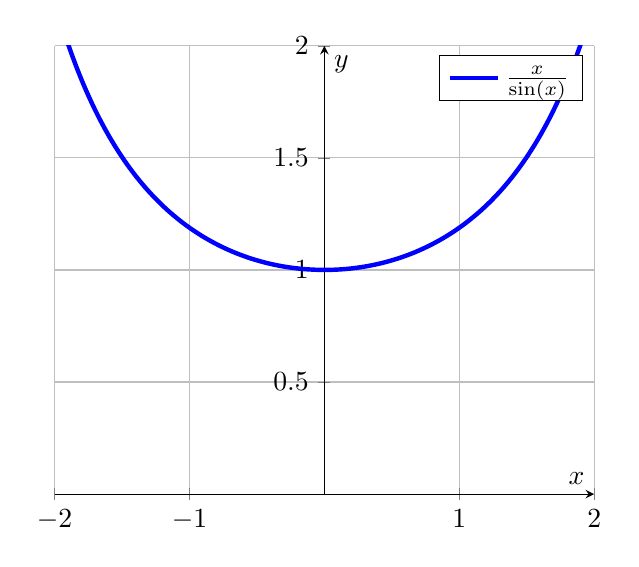
\begin{tikzpicture}[scale=1]
		\begin{axis}[
  			grid=both,
  			xmin=-2,
  			xmax=2,
  			ymin=0,
  			ymax=2,
  			xlabel=$x$,
  			ylabel=$y$,
  			axis lines=center,
  			>=stealth
			]
  		\addplot[
    			domain=-2:2,
    			blue,
    			ultra thick,
    			samples=100,
  			] plot[smooth] {x/sin(deg(x))};
			\legend{$\frac{x}{\sin(x)}$}
		\end{axis}
	\end{tikzpicture}
	\end{center} 
	We can see that  $ 1 \leq \frac{x}{\sin(x)} \leq \frac{\pi}{2}$ for $- \frac{\pi}{2} \leq x \leq \frac{\pi}{2}$; hence, $f(x)$ is well condition.
	However, we notice that $\lim_{x\to 0} cos(x) = 1$ causes catastrophic cancellation for the numerator, which means the algorithm is unstable.
	\item Alternative algorithm: $f(x) = \frac{1-cos(x)}{sin(x)} \times \frac{1+cos(x)}{1+cos(x)} = \frac{sin(x)}{1+cos(x)}$.\\
	Clearly this avoid catastrophic cancellation, when $x$ is close to 1.\\
	Python Program:
	\begin{itemize} [label={}]
	\item \textcolor{orange} {import} math
	\item \textcolor{orange} {def} \textcolor{blue}{q4}():
	\item \ \ \ \  left = - math.pi / 2
	\item \ \ \ \ right = math.pi / 2
	\item  \ \ \ \ \textcolor{orange} {if} (x == 0):
	\item	\ \ \ \	\ \ \ \textcolor{orange} {return} 0
	\item  \ \ \ \ \textcolor{orange} {elif} (x == 0):
	\item \ \ \ \ \ \ \ \ \ numerator = math.sin(x)
	\item \ \ \ \ \ \ \ \ \  denominator = math.cos(x) + 1
	\item	\ \ \ \	\ \ \ \ \textcolor{orange} {return} numerator / denominator
	\item  \ \ \ \ \textcolor{orange} {else}:
	\item	\ \ \ \	\ \ \ \ \textcolor{orange} {return}  \textcolor{orange}{`` not define''}
	 	\end{itemize}	  
	\end{enumerate}
\end{enumerate}
\end{document}